\chapter{Methodology and Setup}
\label{ch:setup}

% There have been debates about the performance
% measure that should be maximized during learning {
% one point of view is that the available data should be
% used to learn all possible perceptual distinctions in the
% real world 

% One of the main issues faced in learning \acrshort{acr:mdp} models is that of deciding on the state space, while one typically does not know the size of the true state space of the real-world process that generated the training data.
%In fact this state space might even have been continuous, while the state space of the model is typically discrete.
%In particular this might form an issue in the planning phase where a reward function needs to be defined to express the goals in the \acrshort{acr:mdp}, for which there may not be a clear one-to-one mapping from real-world states to model states.

% Two approaches:
% - Clustering training data to obtain states
% - Trajectory Clustering

\textbf{Note:} These bullet-points have not been completely updated yet although most are still relevant. Outline should be such that we first discuss the framework for model learning and optimization without considering incomplete data or doing cost-sensitive optimization, which are discussed next ('why and how').
Probably describing the framework should be separated from the application to mobile robot navigation and how it is implemented, which should be described afterwards.

\begin{itemize}
	\item Introduction
	\item Explain high-level algorithm idea?
\end{itemize}

\section{Application}
\label{sec:application}

% 

\begin{itemize}
	\item Mobile robot navigation
	\item Why this application?
	\item Generalization possible to other applications?
\end{itemize}

\section{Exploration Phase}
\label{sec:exploration-phase}

% 

\begin{itemize}
	\item Obtain a dataset of observations, for our application this concerns data about attainable positions of the robot that will be controlled
	\item Under the assumption such a dataset is not yet available to us, this dataset is retrieved in an exploration phase
	\item In this exploration phase, the robot should explore the environment and periodically record information about its current position while aiming to visit all the locations of importance
	\item This exploration phase is (preferably) only carried out once
	\item To obtain a dataset for our tests the exploration phase is carried out in a robot simulator. Should also explain what data is obtained in this exploration.
	\item The overall algorithm is tested for multiple maps/(office-like) environments, which might differ in their dimensions, number of obstacles or `openness'.
	\item To take into account dynamically changing environments to some extent, there are also doors that will be open or closed as time passes.
	\item The simulations are carried out in the Morse simulator, in which the exploration is carried out by an agent that randomly navigates an environment.
\end{itemize}

\section{State Space Acquisition}
\label{sec:state-space-aggregation}

% 

\begin{itemize}
	\item Using exploration data
	\item Unsupervised machine learning to obtain states for an MDP model (various possible methods possible: e.g., kmeans, gmm)
	\item Unknown parameter $\delta$ of the unsupervised machine learning algorithm to be optimized
\end{itemize}

\section{Model and Policy Acquisition}
\label{sec:model-policy-acquisition}

% 

\begin{itemize}
	\item State space obtained as described in previous section
	\item Transition function obtained based on exploration data and state space through the likelihood maximization approach.
	\item For our application the actions are fixed and can either be \textsc{NORTH}, \textsc{EAST}, \textsc{SOUTH}, \textsc{WEST} which makes the robot navigate in the corresponding direction.
	\item Rewards
	\item Timesteps
	\item Policy (various possible `solvers': value iteration, policy iteration)
\end{itemize}

\section{Bayesian Model Optimization}
\label{sec:bayesian-model-optimization}

% 

\begin{itemize}
	\item Optimization of the unknown $\delta$ parameter of the machine learning algorithm for state space aggregation
	\item Evaluation by simulations of the found policy for the given $\delta$ parameter
	\item ...
\end{itemize}

\begin{figure}[t]
	\centering
	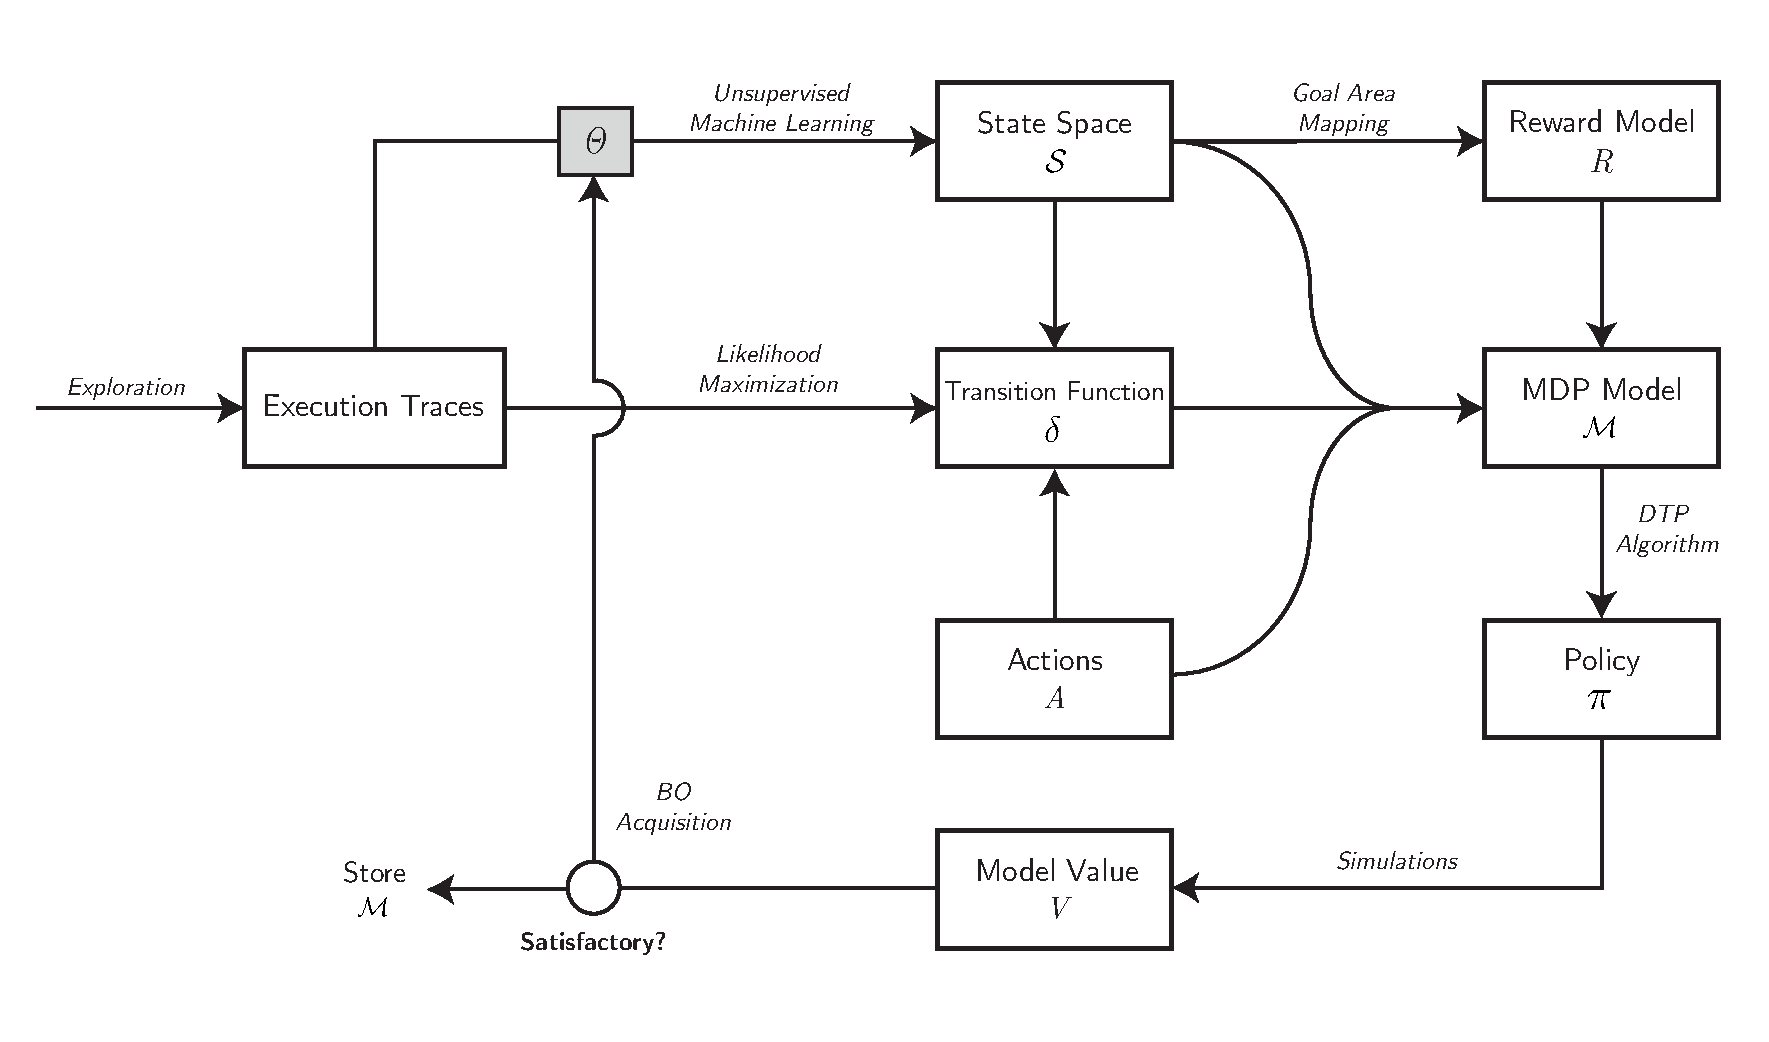
\includegraphics[width=\textwidth]{learning-cycle-complete-v2}
	\caption{Learning Cycle.}
	\label{fig:learning-cycle-complete}
\end{figure}
